\newpage

\section{Example profile}
\label{app:exampleprofile}
\lstinputlisting[language=json,firstnumber=1]{listings/BuyerA.json}
\caption{Preference profile of agent A}

\section*{Figures}
             \begin{figure}[H]
                \centering
                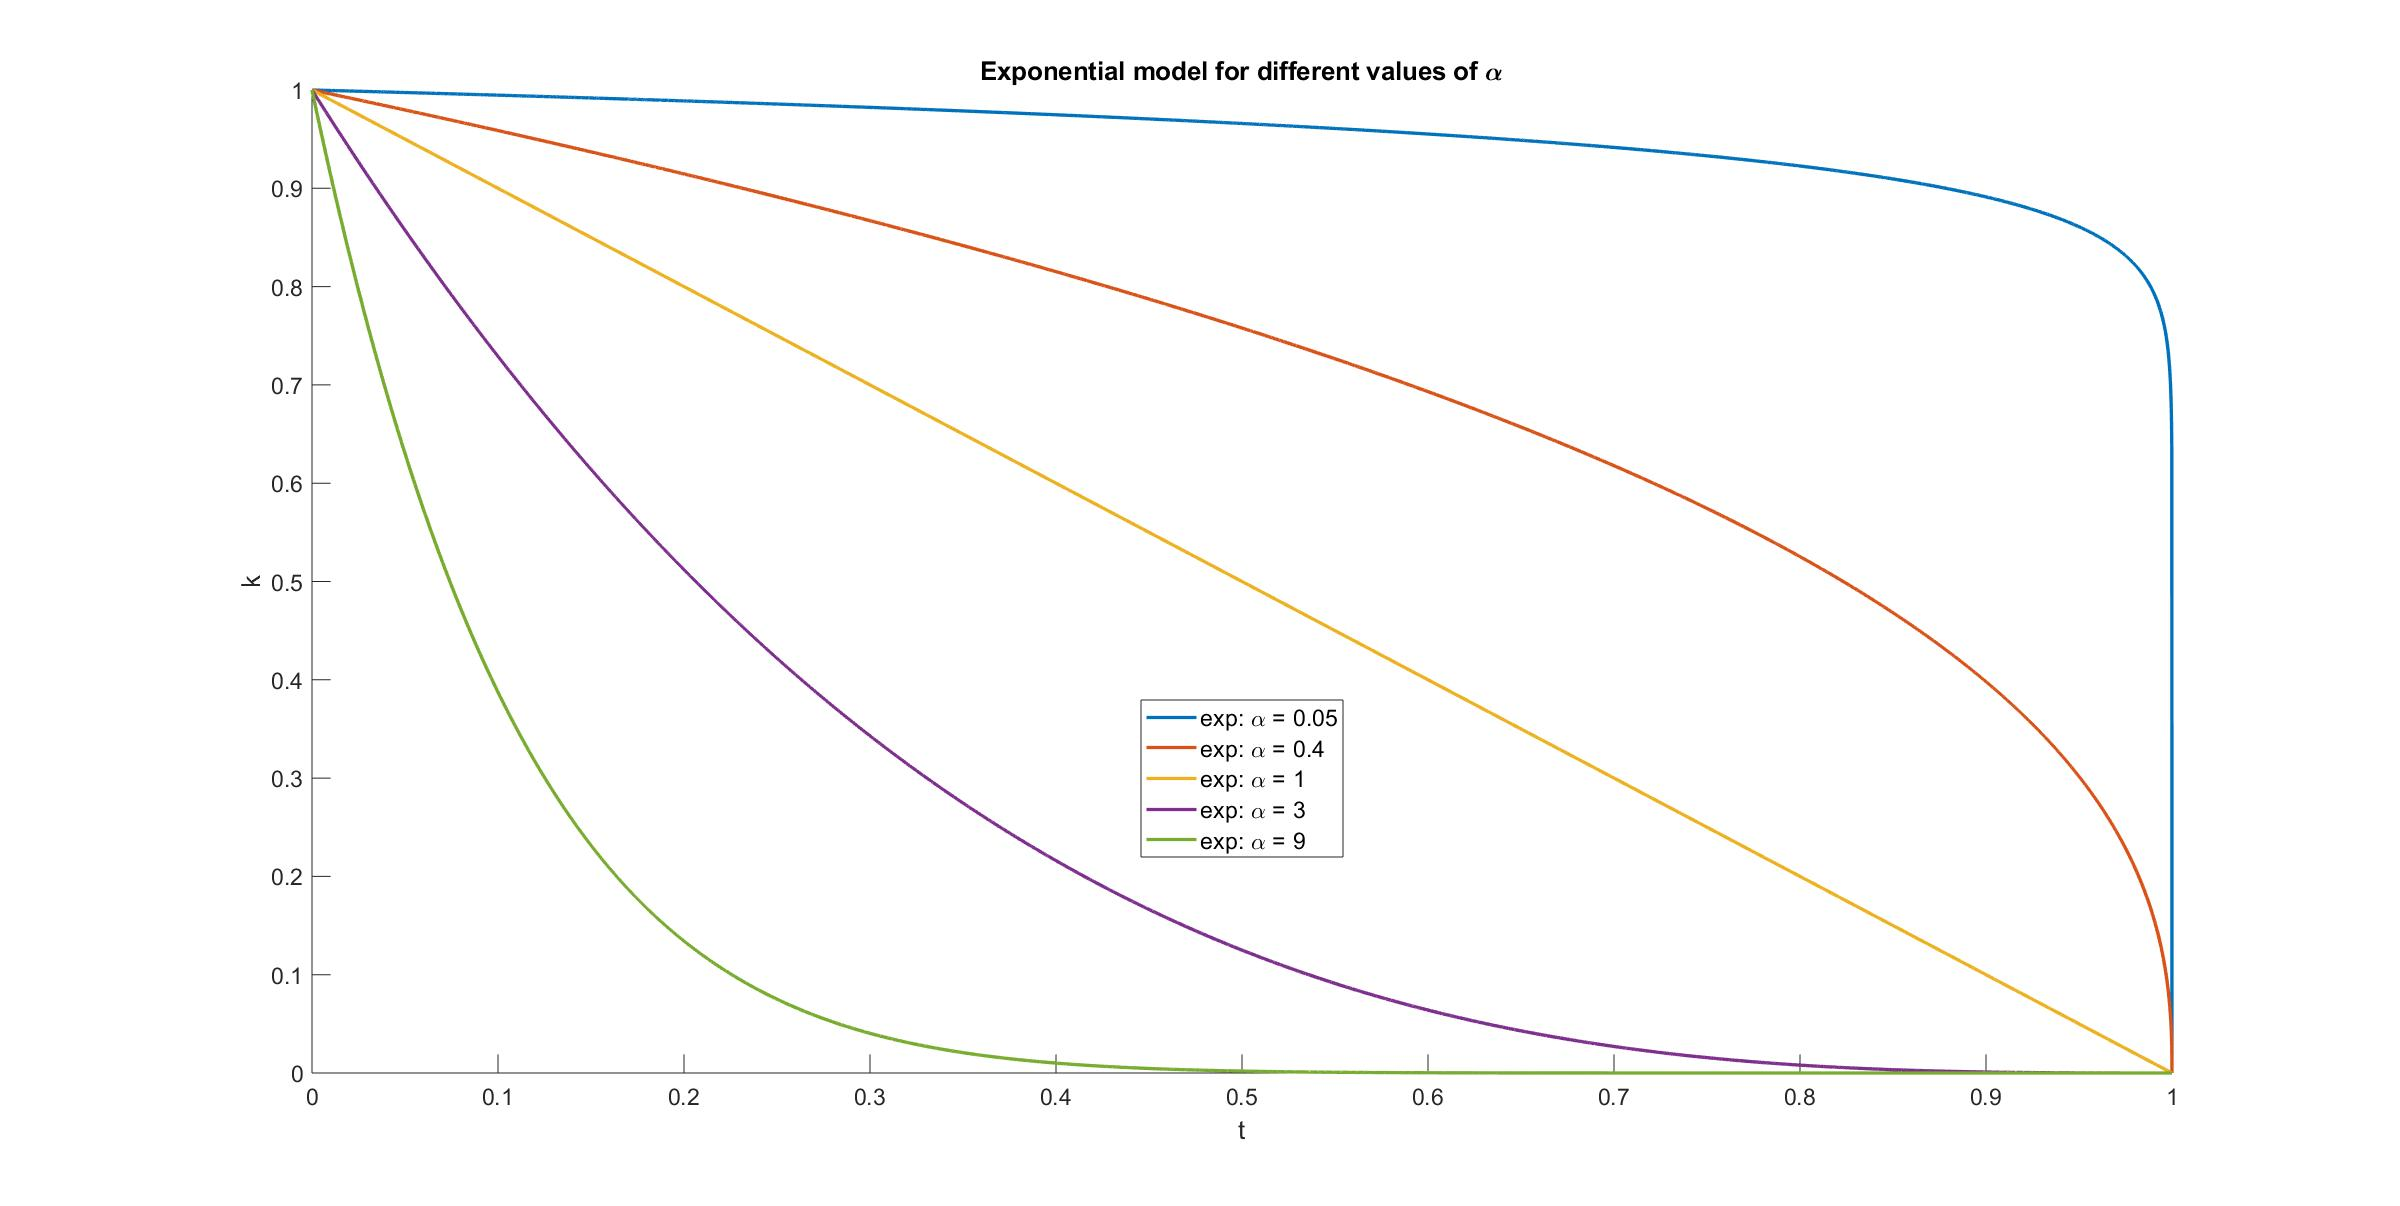
\includegraphics[width=17cm]{figures/Exponential.jpg}
                \caption{Depiction of the exponential conceding strategies for different values of $\alpha$.}
                \label{fig:exp}
            \end{figure}
            
            
            
           \begin{figure}[H]
                \centering
                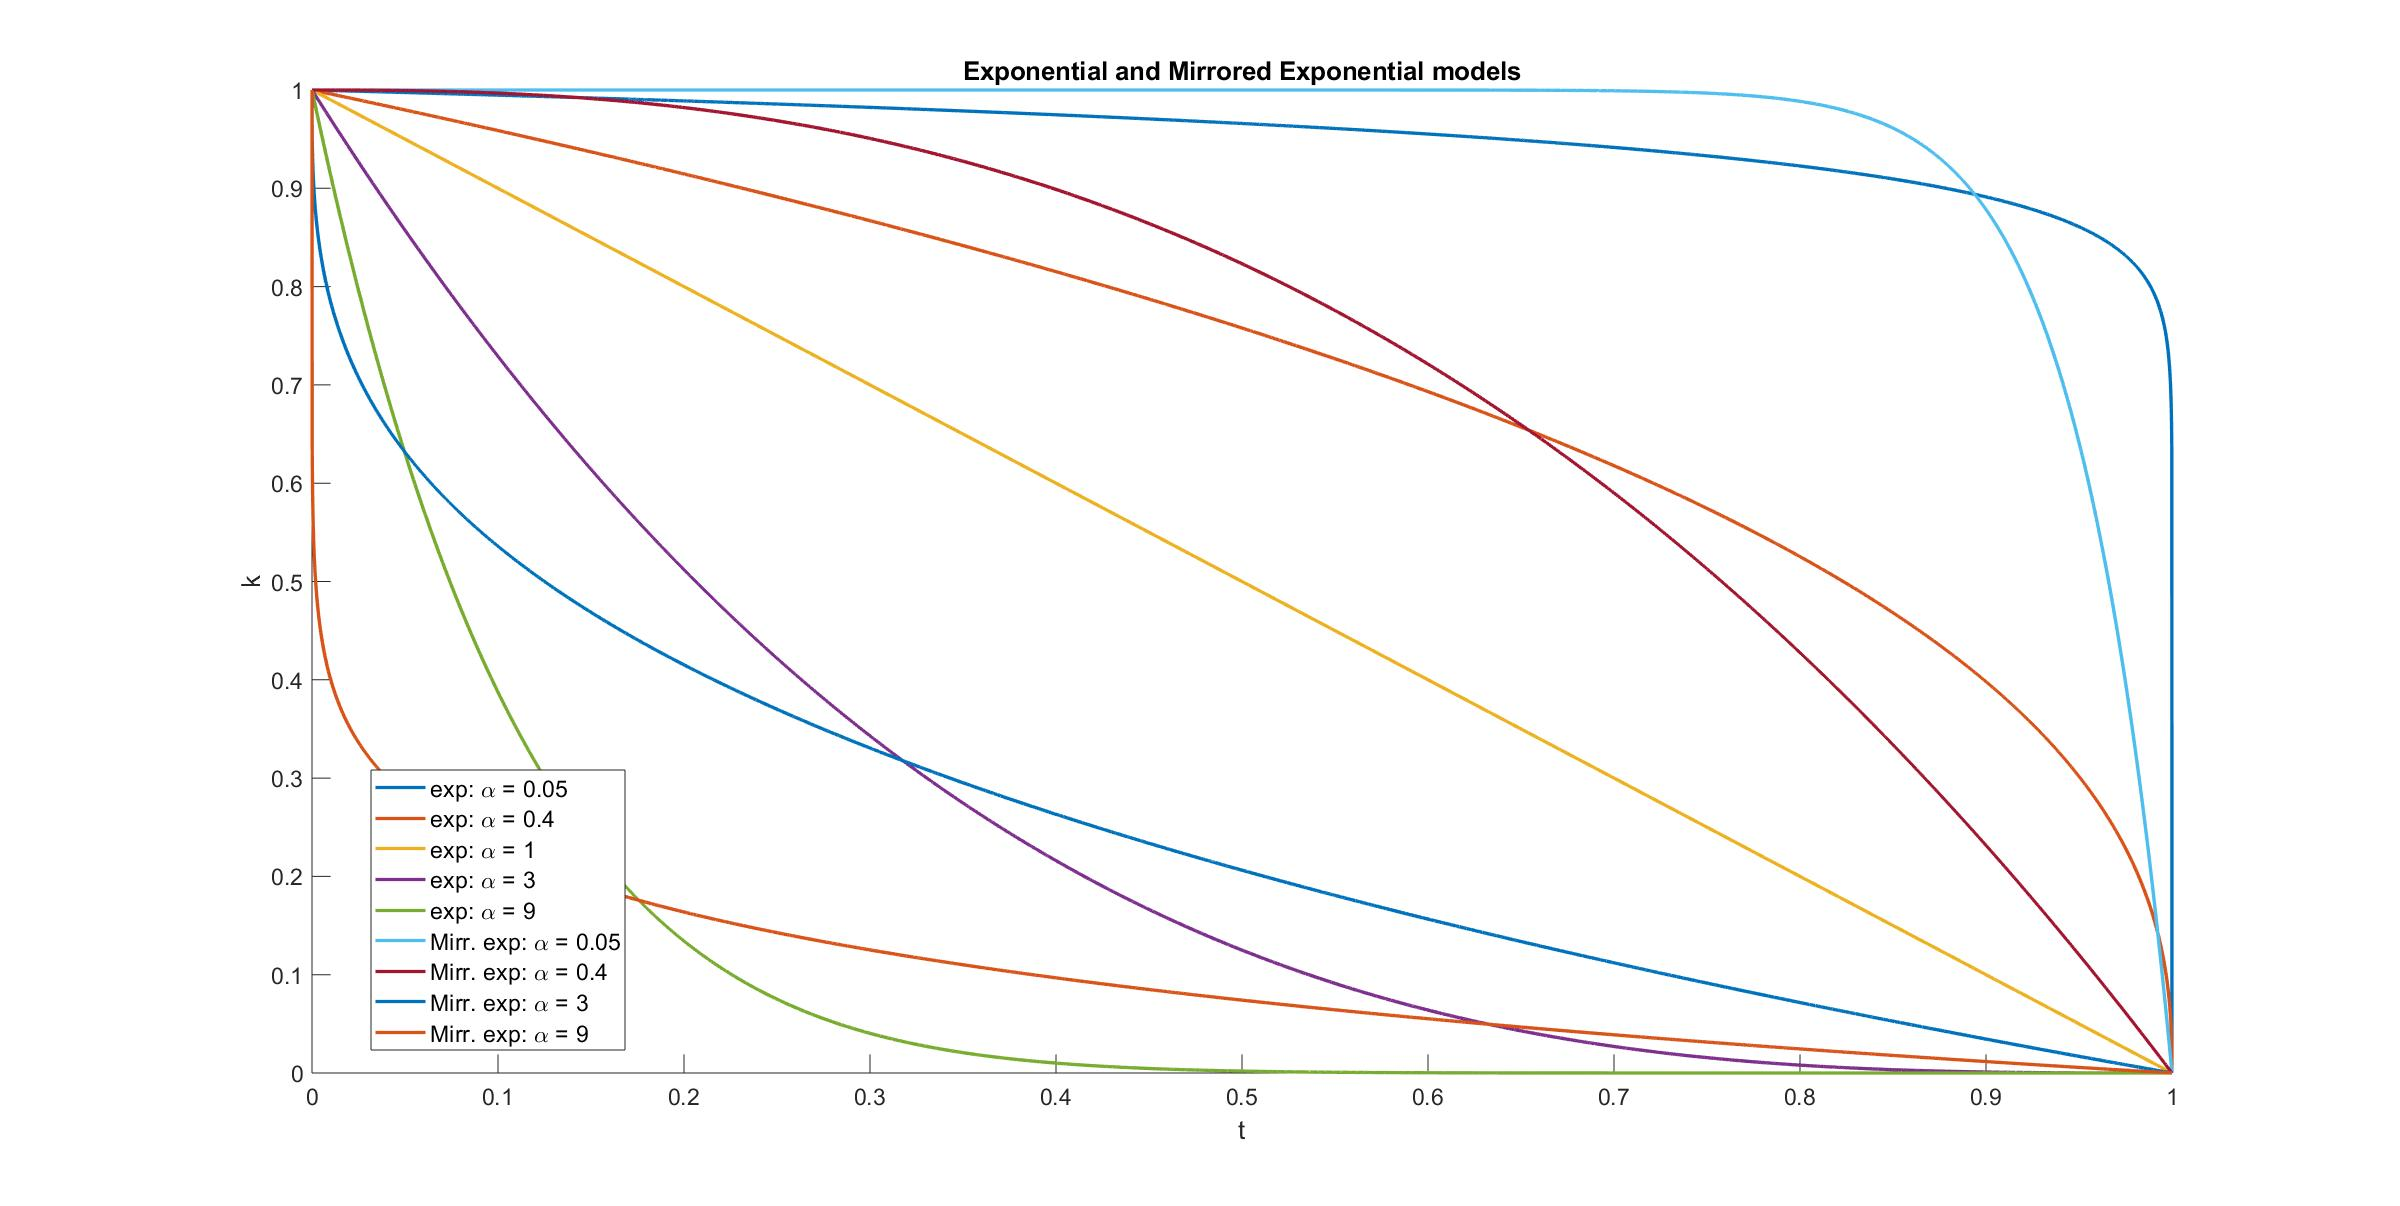
\includegraphics[width=17cm]{figures/combined.jpg}
                \caption{Depiction of the Mirrored Exponential and Exponential conceding strategies for different values of $\alpha$.}
                \label{fig:both}
            \end{figure}
            
            
            \begin{figure}[H]
                \centering
                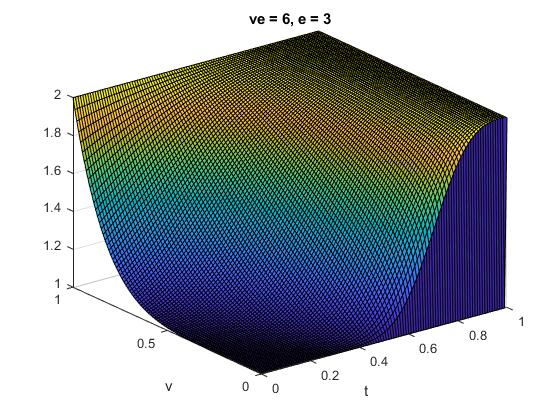
\includegraphics[width=10cm]{figures/powersurface.jpeg}
                \caption{Utility multiplier for a bid with a certain support 'v' over time t. The agent's set values are $\beta$ = 6 and $\alpha$ = 3.}
                \label{fig:powersurface}
            \end{figure} 
            
            
            \begin{figure}[H]
                \centering
                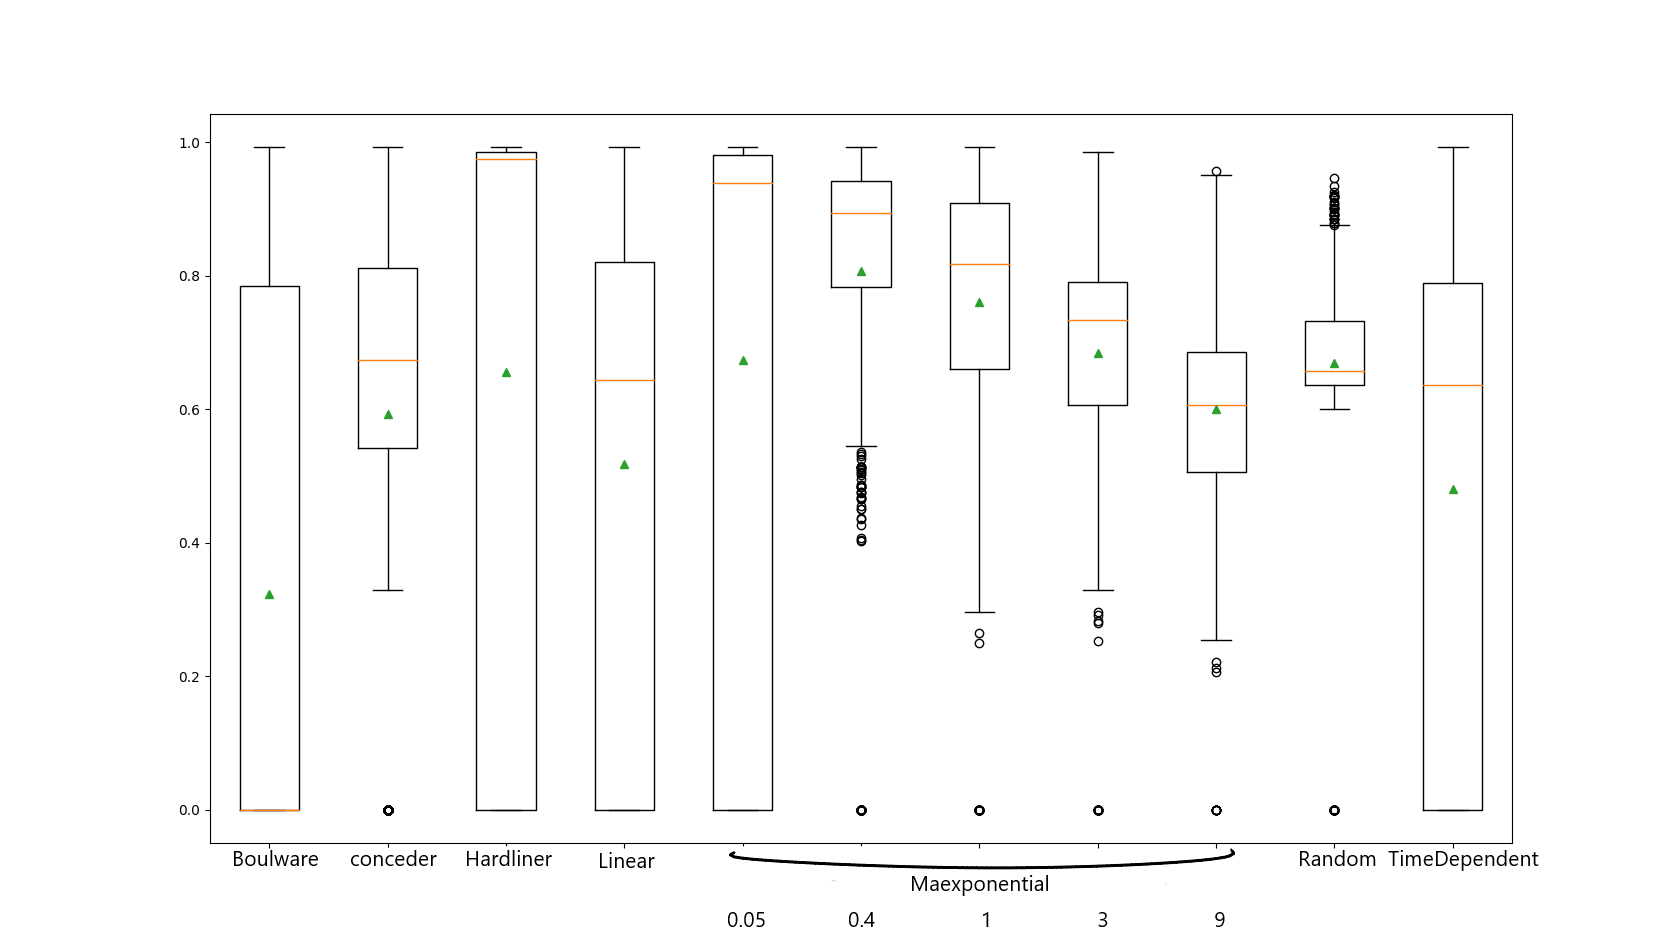
\includegraphics[width=15cm]{figures/Basic_test_1.png}
                \caption{Box plot depicting the utility outcome values for the different parties, after 4000 random sessions. Outcomes without an agreement are included (zero utility).}
                \label{fig:test_1}
            \end{figure}
            
            
            \begin{figure}[H]
                \centering
                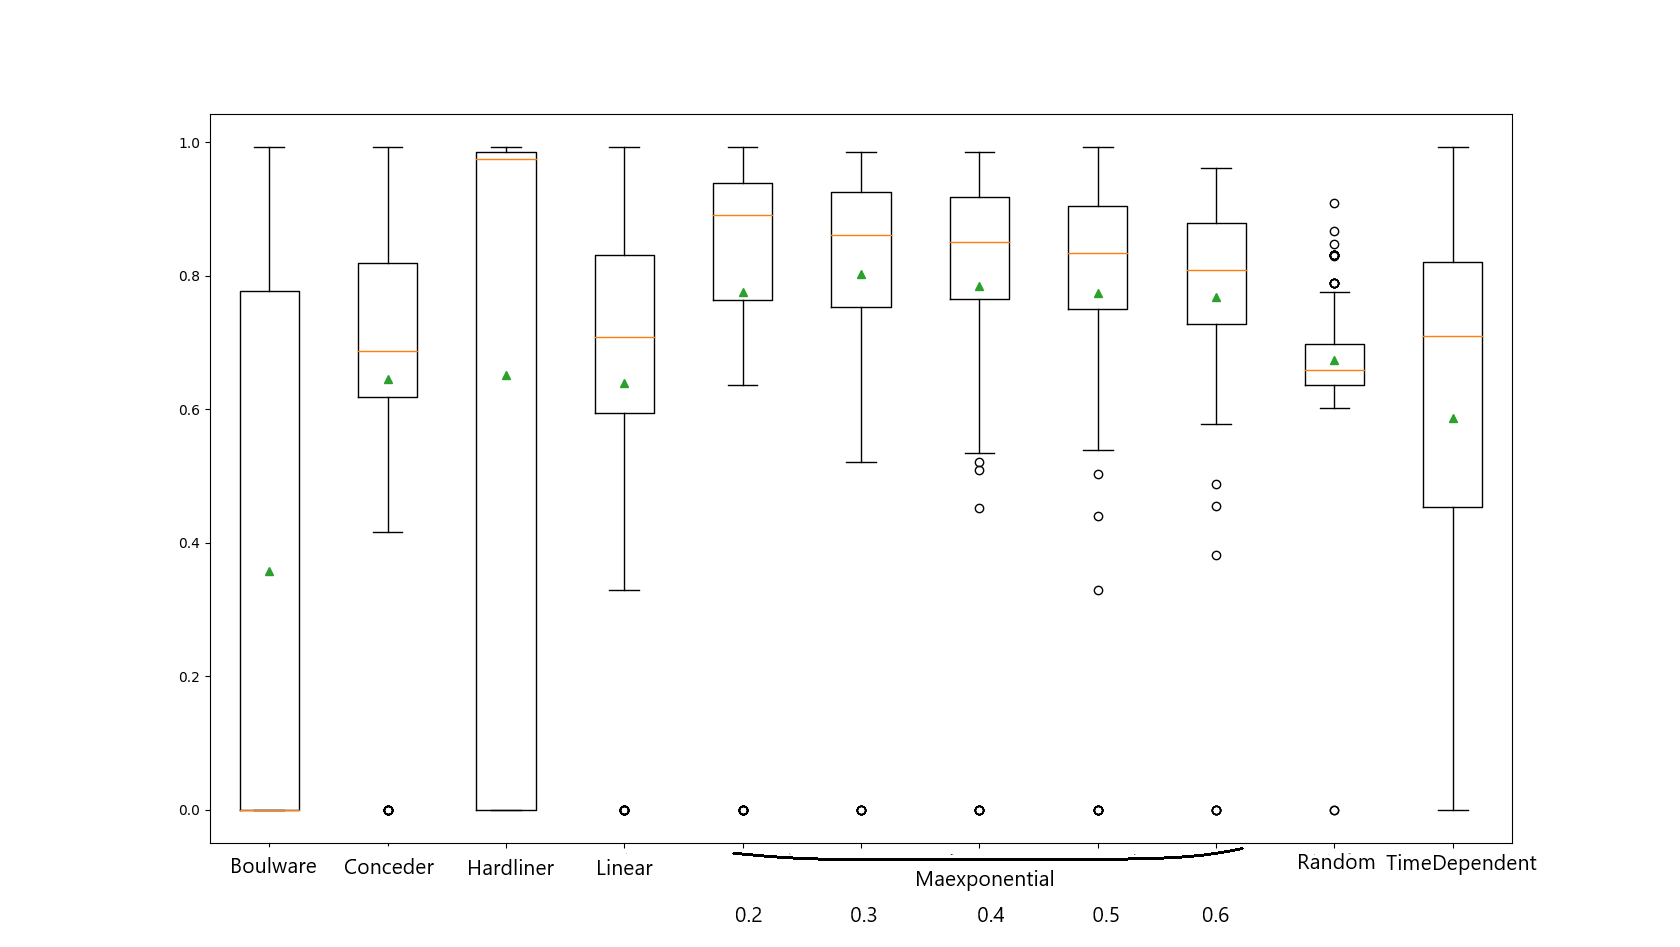
\includegraphics[width=15cm]{figures/Basic_test_2.png}
                \caption{Box plot depicting 400 random sessions with the exponential agents within a smaller range for the exponent (0.2-0.6)}
                \label{fig:test_2}
            \end{figure}
            
            
            \begin{figure}[H]
                \centering
                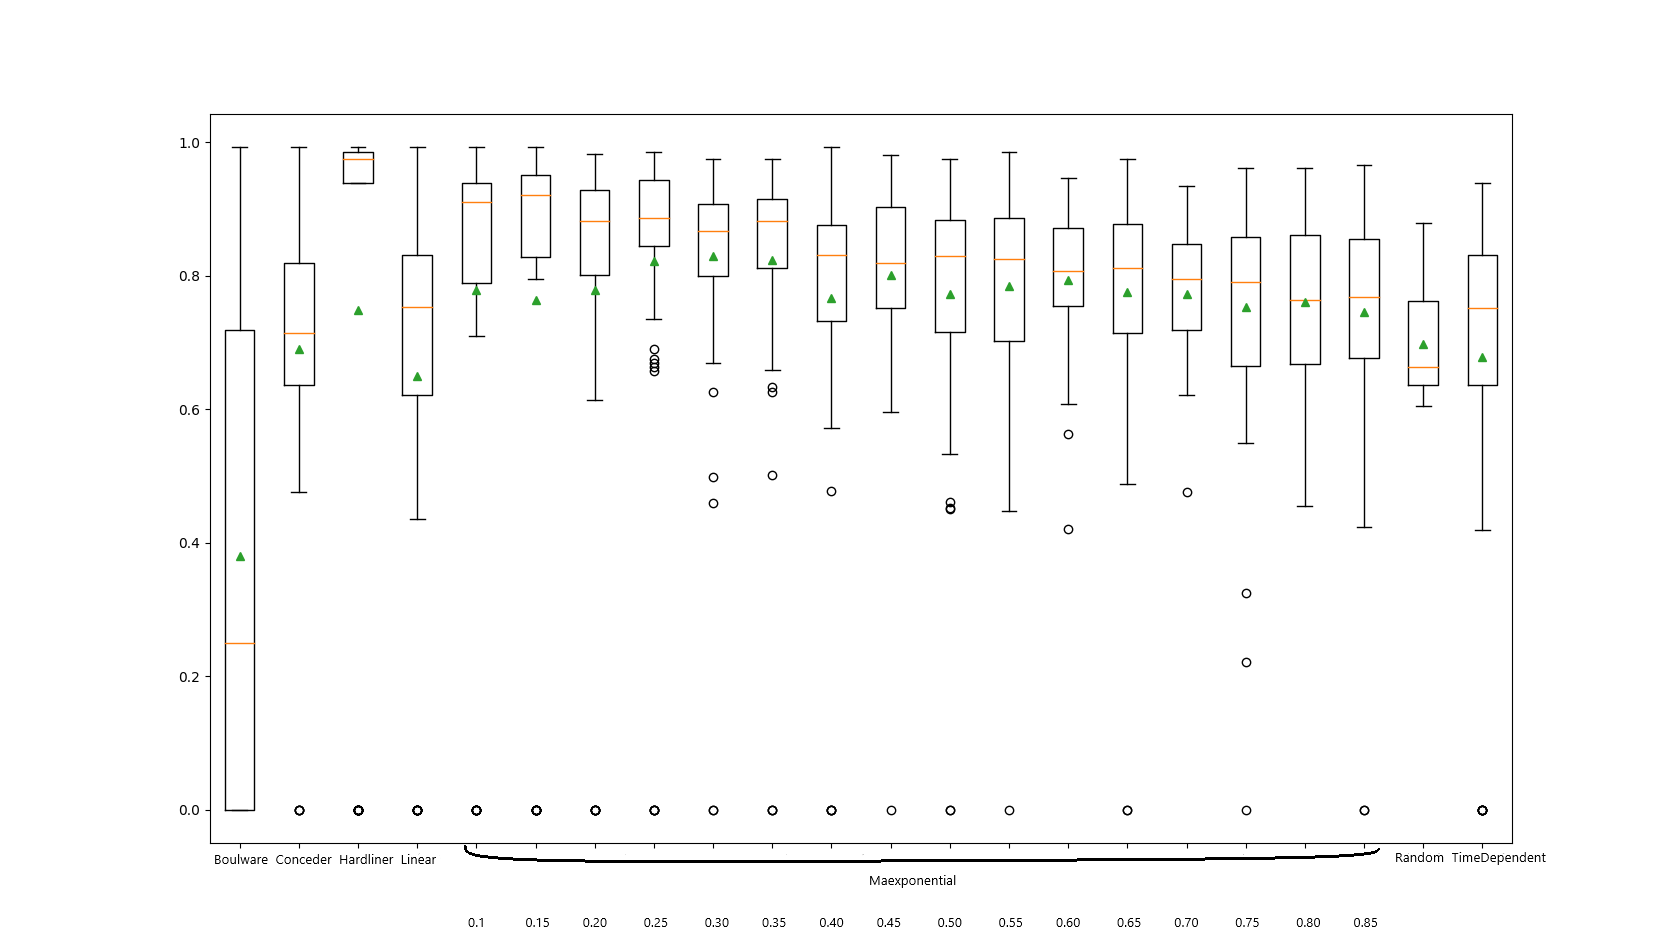
\includegraphics[width=15cm]{figures/Basic_test_3.png}
                \caption{Final box plot depicting the outcome of 400 sessions and $\alpha$ ranging from 0.1 to 0.85 with steps of 0.05.}
                \label{fig:test_3}
            \end{figure}
            
            
            \begin{figure}[H]
                \centering
                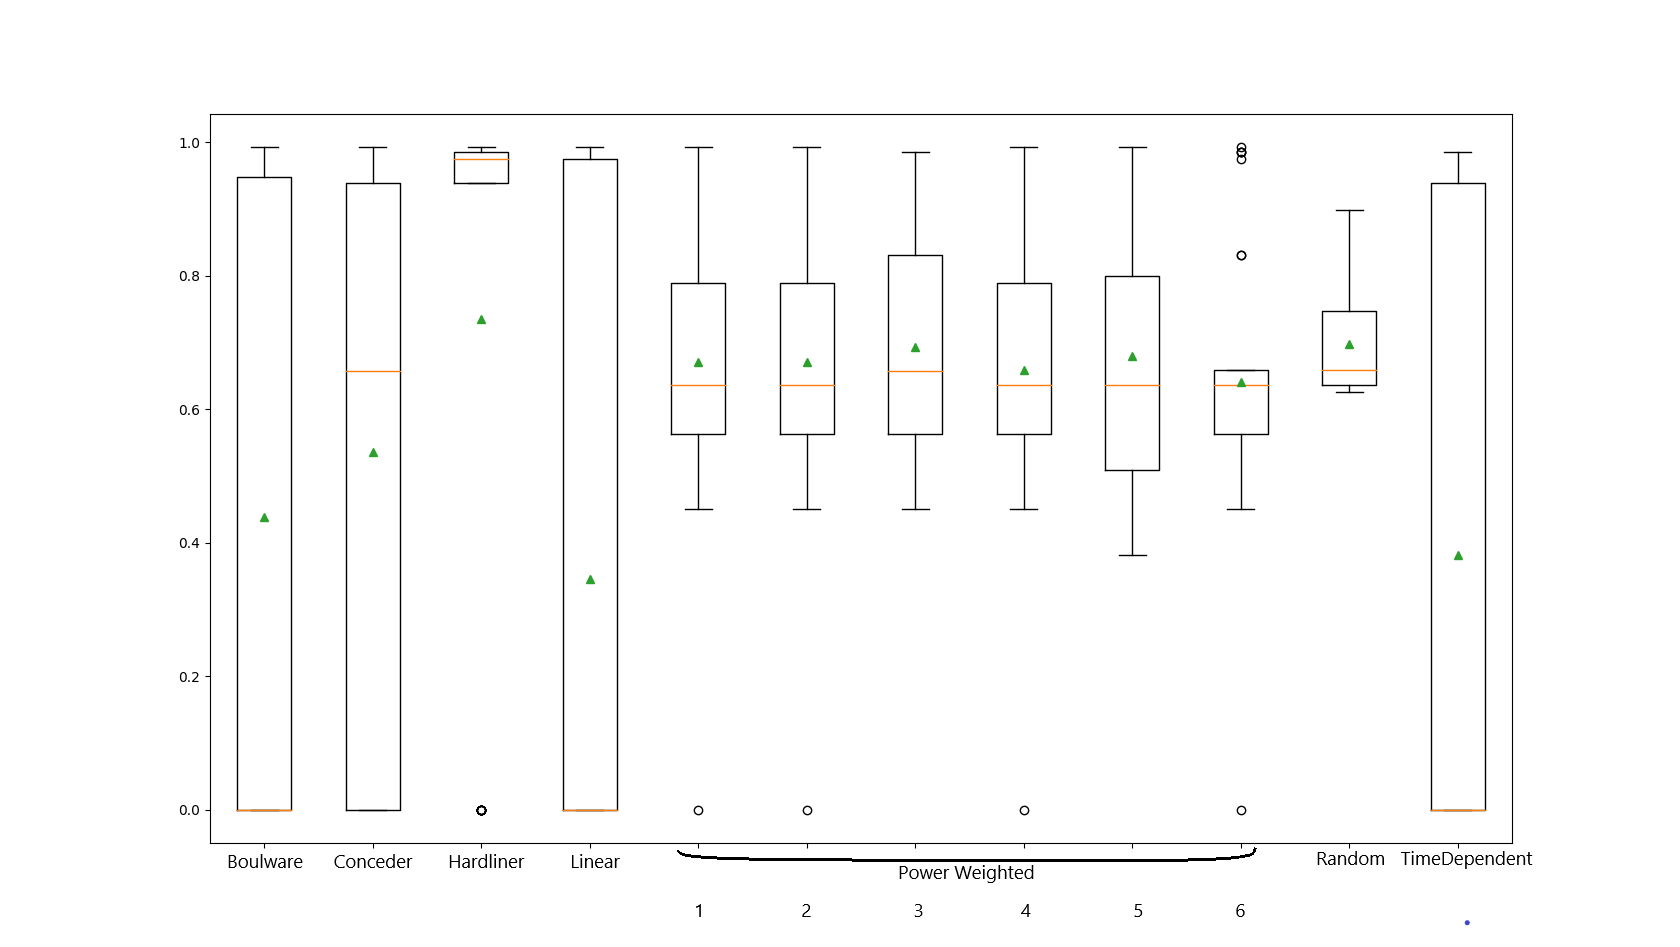
\includegraphics[width=15cm]{figures/Power factor test.png}
                \caption{A box plot depicting a test run with GeniusWeb and power-weighted agents with constant $\alpha = 0.3$ and $\beta$ varying from 1-6.}
                \label{fig:power_factor}
            \end{figure}
            
            
            
            \begin{figure}[H]
                \centering
                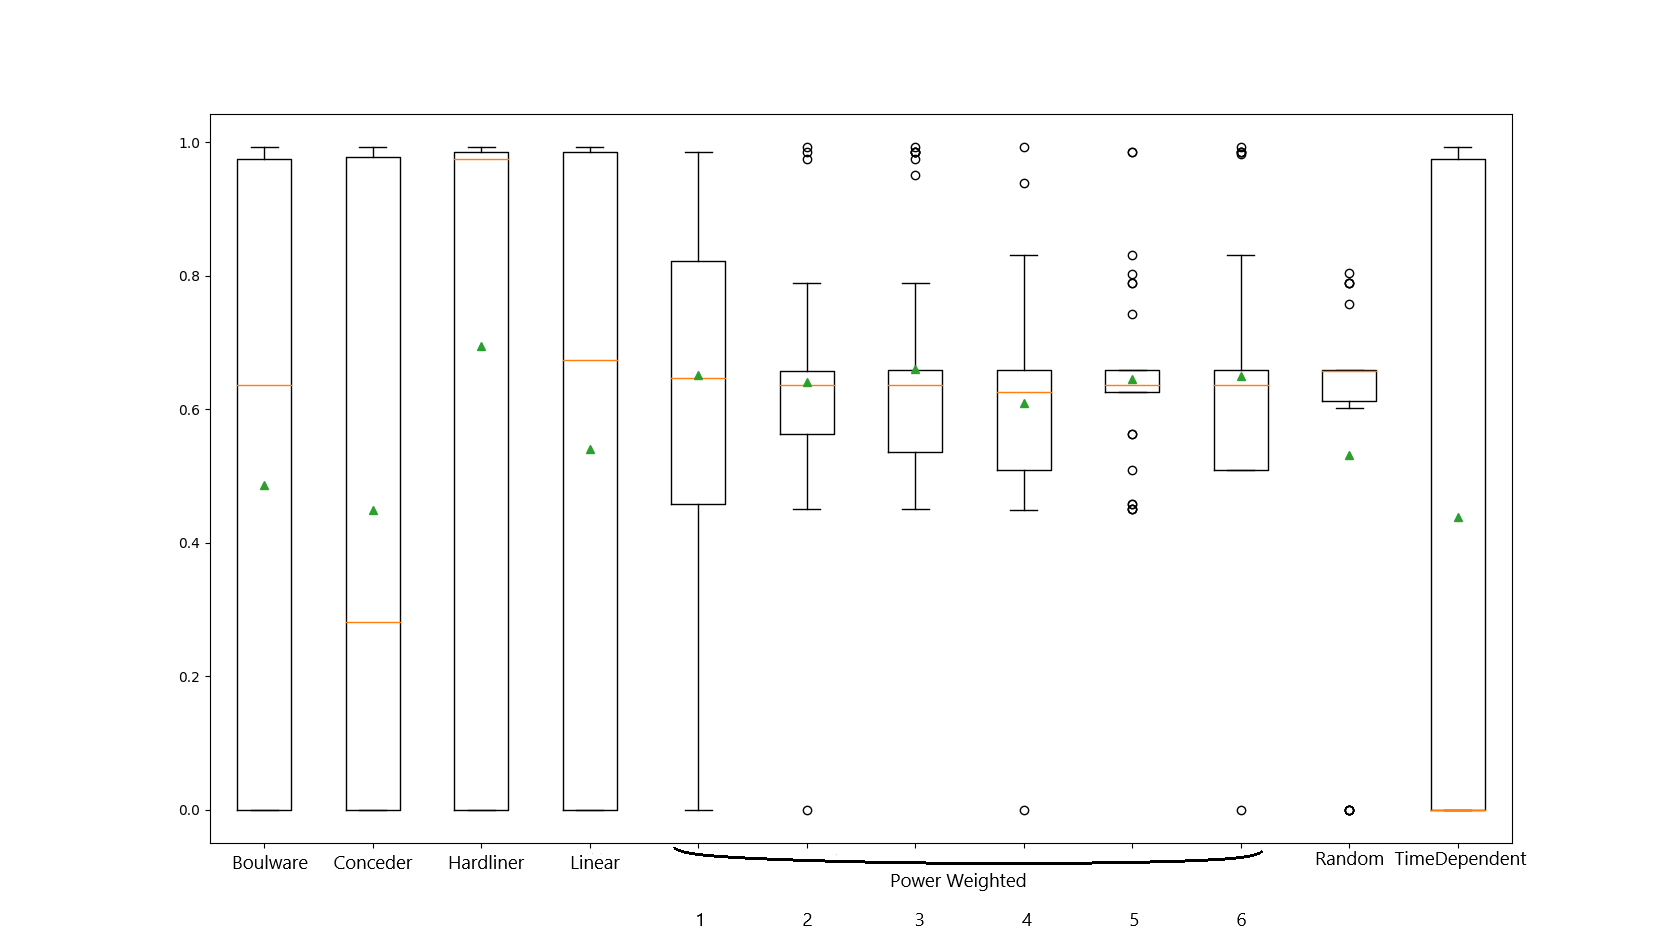
\includegraphics[width=15cm]{figures/Power-Time.png}
                \caption{A box plot depicting a test run with GeniusWeb and power-weighted agents with varying $\alpha$ from 0.2-0.6 and constant $\beta$.}
                \label{fig:power_time}
            \end{figure}